\section{Equation}


Below are two example equations written using LaTeX:

\subsection*{Equation 1}

\begin{equation}
7 \left(
\pi + \int_{0}^{1}
\frac{x^{4}(1-x)^{4}}{1+x^{2}}
\right) = 22
\end{equation}


\subsection*{Equation 2}

\begin{equation}
\end{equation}
\begin{center}

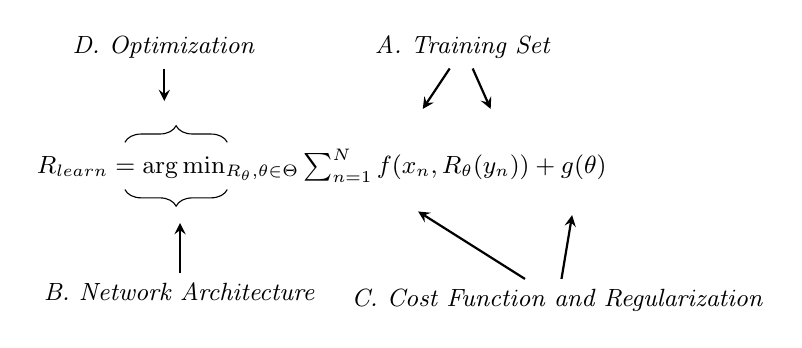
\begin{tikzpicture}[>=stealth, every node/.style={font=\small}]

% Main equation
\node (eq) at (0,0) {$
R_{\text{learn}}
=
\arg\min_{R_\theta,\theta \in \Theta}
\sum_{n=1}^{N}
f(x_n, R_\theta(y_n))
+
g(\theta)
$};


% Labels
\node (opt) at (-2,1.5) {\textit{D. Optimization}};
\node (optpoint) at (-2,0.7) {};
\draw[->, thick] (opt) -- (optpoint);

\node (train) at (1.8,1.5) {\textit{A. Training Set}};
\node (opoint) at (1.2,0.6) {};
\draw[->, thick] (train) -- (opoint);
\node (ooint) at (2.2,0.6) {};
\draw[->, thick] (train) -- (ooint);


\node (arch) at (-1.8,-1.6) {\textit{B. Network Architecture}};
\node (oppoint) at (-1.8,-0.6) {};
\draw[->, thick] (arch) -- (oppoint);

\node (cost) at (3.0,-1.7) {\textit{C. Cost Function and Regularization}};
\node (oint) at (1.1,-0.5) {};
\draw[->, thick] (cost) -- (oint);
\node (oint) at (3.2,-0.5) {};
\draw[->, thick] (cost) -- (oint);



% Arrows

% Curly brace above argmin
\draw[decorate,decoration={brace,amplitude=6pt}]
(-2.5,0.3) -- (-1.2,0.3);

% Curly brace below parameters
\draw[decorate,decoration={brace,mirror,amplitude=6pt}]
(-2.5,-0.3) -- (-1.2,-0.3);

\end{tikzpicture}

\end{center}
\end{equation}